\RequirePackage{amsmath}
\RequirePackage{fix-cm}
\documentclass{svmono}

\def\ColoredLinks{}
%%%%%%%%%%%%%%%%%%%%%%%%%%%%%%%%%%%%%%%%%%%
% Alexanders Standardmacros - Version 3.0 %
%%%%%%%%%%%%%%%%%%%%%%%%%%%%%%%%%%%%%%%%%%%





%%%%%%%%%%%%%%%%%%%%%%%%%%%%%%%%%%%%%%%%%%%%%%%%
%  Farben für Links definieren                 %
%%%%%%%%%%%%%%%%%%%%%%%%%%%%%%%%%%%%%%%%%%%%%%%%

\ifdefined\ColoredLinks
  \def\linkColorLinkR{0}
  \def\linkColorLinkG{0}
  \def\linkColorLinkB{0.55}
	\def\linkColorCiteR{0}
  \def\linkColorCiteG{0}
  \def\linkColorCiteB{0.55}
	\def\linkColorUrlR{0}
  \def\linkColorUrlG{0}
  \def\linkColorUrlB{0.55}
\else
  \def\linkColorLinkR{0}
  \def\linkColorLinkG{0}
  \def\linkColorLinkB{0}
	\def\linkColorCiteR{0.3}
  \def\linkColorCiteG{0.3}
  \def\linkColorCiteB{0.3}
	\def\linkColorUrlR{0}
  \def\linkColorUrlG{0}
  \def\linkColorUrlB{0}
\fi





%%%%%%%%%%%%%%%%%%%%%%%%%%%%%%%%%%%%%%%%%%%%%%%%
%  Packages einbinden                          %
%%%%%%%%%%%%%%%%%%%%%%%%%%%%%%%%%%%%%%%%%%%%%%%%

%\usepackage{makeidx} - unterschägt manchmal Einträge
\usepackage{imakeidx} % Speziellen Features eigentlicht nicht verwendet, aber hat die makeidx-Fehler nicht
\usepackage[utf8]{inputenc}
\usepackage{amssymb}
\usepackage[ngerman]{babel}
\usepackage{epsf}
\usepackage[dvips]{rotating}
\usepackage{amsmath,amsfonts}
\usepackage[amsmath,thmmarks,noconfig]{ntheorem}
\usepackage{nameref}
\usepackage{hycolor}
\usepackage{hyperxmp}
\usepackage{hyperref}
\hypersetup{pdfauthor={Alexander Herzog},
            pdftitle={Warteschlangensimulator - Kurzeinführung},
            %pdfsubject={},
            %pdfkeywords={},
            pdfproducer={LaTeX},
            pdfcreator={pdfLaTeX},
						pdfcopyright={Copyright Alexander Herzog},
						pdfcontactcity={Clausthal-Zellerfeld},
						pdfcontactpostcode={38678},
						pdfcontactcountry={Deutschland},
						pdfcontactemail={alexander.herzog@tu-clausthal.de},
						pdfcontacturl={https://www.simzentrum.de,https://www.tu-clausthal.de},
						pdflang={de},
						bookmarksnumbered,
						colorlinks=true,
						filecolor=[rgb]{0,0,0},  % \href-Links nicht hervorheben
						linkcolor=[rgb]{\linkColorLinkR,\linkColorLinkG,\linkColorLinkB},
						citecolor=[rgb]{\linkColorCiteR,\linkColorCiteG,\linkColorCiteB},
						urlcolor=[rgb]{\linkColorUrlR,\linkColorUrlG,\linkColorUrlB} %\url{}, nur für E-Mail-Link genutzt
					}
\expandafter\def\expandafter\UrlBreaks\expandafter{\UrlBreaks
  \do\a\do\b\do\c\do\d\do\e\do\f\do\g\do\h\do\i\do\j
  \do\k\do\l\do\m\do\n\do\o\do\p\do\q\do\r\do\s\do\t
  \do\u\do\v\do\w\do\x\do\y\do\z\do\A\do\B\do\C\do\D
  \do\E\do\F\do\G\do\H\do\I\do\J\do\K\do\L\do\M\do\N
  \do\O\do\P\do\Q\do\R\do\S\do\T\do\U\do\V\do\W\do\X
  \do\Y\do\Z}
\usepackage{float}
\usepackage{fancyvrb}
\restylefloat{figure}
\restylefloat{table}
\usepackage{sectsty}
%\allsectionsfont{\fontfamily{cmss}\selectfont} - das führt zu Type 3 Fonts
\allsectionsfont{\sffamily\selectfont}
\usepackage{framed}
\usepackage[toc,page]{appendix}
\renewcommand\appendixname{Anhang}
\let\appendixtocname\appendixname\let\appendixpagename\appendixname
\usepackage[T1]{fontenc} % aus der pdf kopierbare Umlaute
\usepackage{eurosym}
\usepackage{longtable}

\usepackage{graphicx}
\usepackage[export]{adjustbox}




%%%%%%%%%%%%%%%%%%%%%%%%%%%%%%%%%%%%%%%%%%%%%%%%
%  Rotierte Tabellenüberschriften              %
%%%%%%%%%%%%%%%%%%%%%%%%%%%%%%%%%%%%%%%%%%%%%%%%

\usepackage{adjustbox}
\usepackage{array}
\usepackage{booktabs}
\usepackage{multirow}

\newcolumntype{R}[2]{%
    >{\adjustbox{angle=#1,lap=\width-(#2)}\bgroup}%
    l%
    <{\egroup}%
}
\newcommand*\rot{\multicolumn{1}{|R{90}{1em}|}}





%%%%%%%%%%%%%%%%%%%%%%%%%%%%%%%%%%%%%%%%%%%%%%%%
%  Symbole definieren                          %
%%%%%%%%%%%%%%%%%%%%%%%%%%%%%%%%%%%%%%%%%%%%%%%%

\newcommand{\setH}{\mathbb{H}}
\newcommand{\setC}{\mathbb{C}}
\newcommand{\setR}{\mathbb{R}}
\newcommand{\setQ}{\mathbb{Q}}
\newcommand{\setZ}{\mathbb{Z}}
\newcommand{\setN}{\mathbb{N}}
\newcommand{\comp}{\complement}
\newcommand{\Umg}{{\cal U}}

\newcommand{\calA}{{\cal A}}
\newcommand{\calB}{{\cal B}}
\newcommand{\calC}{{\cal C}}
\newcommand{\calD}{{\cal D}}
\newcommand{\calE}{{\cal E}}
\newcommand{\calF}{{\cal F}}
\newcommand{\calG}{{\cal G}}
\newcommand{\calH}{{\cal H}}
\newcommand{\calI}{{\cal I}}
\newcommand{\calJ}{{\cal J}}
\newcommand{\calK}{{\cal K}}
\newcommand{\calL}{{\cal L}}
\newcommand{\calM}{{\cal M}}
\newcommand{\calN}{{\cal N}}
\newcommand{\calO}{{\cal O}}
\newcommand{\calP}{{\cal P}}
\newcommand{\calQ}{{\cal Q}}
\newcommand{\calR}{{\cal R}}
\newcommand{\calS}{{\cal S}}
\newcommand{\calT}{{\cal T}}
\newcommand{\calU}{{\cal U}}
\newcommand{\calV}{{\cal V}}
\newcommand{\calW}{{\cal W}}
\newcommand{\calX}{{\cal X}}
\newcommand{\calY}{{\cal Y}}
\newcommand{\calZ}{{\cal Z}}

\def\arccot{\mathop{\rm arccot}}
\def\Arcoth{\mathop{\rm Arcoth}}
\def\Arsinh{\mathop{\rm Arsinh}}
\def\Artanh{\mathop{\rm Artanh}}
\def\Arcosh{\mathop{\rm Arcosh}}

\def\d{{\rm d}}
\def\dx{\d x}
\def\dy{\d y}
\def\dz{\d z}
\def\dt{\d t}
\def\euler{\mathrm{e}}

\def\id{{\rm id}}
\def\Kern{{\rm Kern}}

\def\ra{\Rightarrow}

\def\oversym#1#2{\mathop{#1}\limits^{#2}}
\def\Inneres#1{\oversym{#1}\circ}


\def\TO#1{\oversym\longrightarrow{#1}}
\def\RA#1{\oversym\Longrightarrow{#1}}
\def\IFF#1{\oversym\iff{#1}}
\def\gleich#1{\oversym={#1}}

\def\oBdA{o.\,B.\,d.\,A.\ }

\renewcommand{\qed}{\begin{flushright} $\square$ \end{flushright}}

\def\Definition#1{{\bf #1}}

\def\E{{\bf E}}
\def\Var{{\bf Var}}
\def\Std{{\bf Std}}
\def\CV{{\bf CV}}
\def\SCV{{\bf SCV}}





%%%%%%%%%%%%%%%%%%%%%%%%%%%%%%%%%%%%%%%%%%%%%%%%
%  Umgebungen definieren                       %
%%%%%%%%%%%%%%%%%%%%%%%%%%%%%%%%%%%%%%%%%%%%%%%%

%\theoremstyle{changebreak}
%\theoremheaderfont{\normalfont\bfseries}
%\theoremseparator{:}
%\theoremsymbol{}
%\newtheorem{definition}{Definition}[chapter]
%\newtheorem{satz}[definition]{Satz}
%\newtheorem{hilfssatz}[definition]{Hilfssatz}
%\newtheorem{lemma}[definition]{Lemma}
%\newtheorem{beispiel}[definition]{Beispiel}
%\newtheorem{beispiele}[definition]{Beispiele}
%\newtheorem{bezeichnung}[definition]{Bezeichnung}
%\theorembodyfont{\rmfamily}
%\newtheorem{bemerkung}[definition]{Bemerkung}
%\newtheorem{vereinbarung}[definition]{Vereinbarung}
%\newtheorem{folgerung}[definition]{Folgerung}
%\theoremheaderfont{\normalfont\bfseries}
%\theoremstyle{nonumberchangebreak}
%\theorembodyfont{\rmfamily}
%\theoremsymbol{$\blacksquare$}
%\newtheorem{beweis}{Beweis}
%\theoremsymbol{}





%%%%%%%%%%%%%%%%%%%%%%%%%%%%%%%%%%%%%%%%%%%%%%%%
%  Standard epsilon durch schöneres ersetzen   %
%%%%%%%%%%%%%%%%%%%%%%%%%%%%%%%%%%%%%%%%%%%%%%%%

\def\epsilon{\varepsilon}





%%%%%%%%%%%%%%%%%%%%%%%%%%%%%%%%%%%%%%%%%%%%%%%%
%  Verbatim-Umgebungen für verschiedene Zwecke %
%%%%%%%%%%%%%%%%%%%%%%%%%%%%%%%%%%%%%%%%%%%%%%%%

\DefineVerbatimEnvironment{ExcelVerbatim}{Verbatim}{frame=single,label=Excel-Befehl,fontsize=\small}
\DefineVerbatimEnvironment{ExcelVerbatimWithMath}{Verbatim}{frame=single,label=Excel-Befehl,commandchars=\\\{\},codes={\catcode`$=3\catcode`^=7},fontsize=\small}
\DefineVerbatimEnvironment{ExcelVerbatimWithFormat}{Verbatim}{frame=single,label=Excel-Befehl,fontsize=\small,commandchars=\\\{\}}
\DefineVerbatimEnvironment{RVerbatim}{Verbatim}{frame=single,label=R-Code,fontsize=\small}
\DefineVerbatimEnvironment{ExcelMacroVerbatim}{Verbatim}{frame=single,label=Excel-Makro,fontsize=\small} % ,numbers=left
\DefineVerbatimEnvironment{ExcelMarcroVerbatimWithMath}{Verbatim}{frame=single,label=Excel-Makro,commandchars=\\\{\},codes={\catcode`$=3\catcode`^=7},fontsize=\small}
\DefineVerbatimEnvironment{ExcelMacroVerbatimWithFormat}{Verbatim}{frame=single,label=Excel-Makro,fontsize=\small,commandchars=\\\{\}}
\newcommand{\sub}[2]{{#1_#2}}

\newcommand{\newlinesymbol}{\rotatebox[origin=c]{270}{$\curvearrowright$}}





%%%%%%%%%%%%%%%%%%%%%%%%%%%%%%%%%%%%%%%%%%%%%%%%
%  Formatierungen                              %
%%%%%%%%%%%%%%%%%%%%%%%%%%%%%%%%%%%%%%%%%%%%%%%%

%\def\emphasis#1{\textbf{#1}}
%\def\emphasisBFOnly#1{\textbf{#1}}
\def\emphasis#1{\emph{#1}}
\def\emphasisBFOnly#1{#1}

\def\emphasisIT#1{\textit{#1}}
\def\emphasisEnglish#1{\textit{#1}}

%\font\deutschfont=suet14
%\def\deutsch#1{\hbox{\deutschfont #1}}

\parindent0pt
\parskip5pt

%\oddsidemargin4.6mm
%\evensidemargin-5.4mm
%\textwidth160mm
\usepackage{xcolor}
\usepackage{lmodern}
\usepackage{wrapfig}
\textwidth160mm
\textheight220mm
\oddsidemargin0mm
\evensidemargin0mm
\topmargin0mm

\def\cmd#1{\textbf{"\texttt{#1}"}}
\def\cm#1{\textbf{\texttt{#1}}}

\begin{document}

\thispagestyle{empty}
\vskip5cm {\Huge\textbf{Short introduction to \vskip.1cm Warteschlangensimulator}}
\vskip.5cm \hrule
\vskip.5cm {\large \textsc{Alexander Herzog} (\href{mailto:alexander.herzog@tu-clausthal.de}{alexander.herzog@tu-clausthal.de})}
\IfFileExists{../../Warteschlangennetz-mittel.png}{
\vskip2cm \centerline{\fbox{\includegraphics[width=16cm]{../../Warteschlangennetz-mittel.png}}}
}{}
\vskip2cm {\color{gray}
This tutorial refers to version 4.6.0
 of Warteschlangensimulator.\\
Download address: \href{https://github.com/A-Herzog/Warteschlangensimulator/}{https://github.com/A-Herzog/Warteschlangensimulator/}.
}
\renewcommand{\thepage}{\roman{page}}

{
\clearpage
\pdfbookmark{Table of contents}{Table of contents}
\begingroup \let\cleardoublepage\relax \tableofcontents \endgroup
}



\chapter{Introduction}

\renewcommand{\thepage}{\arabic{page}}
\setcounter{page}{1}

The Warteschlangensimulator is a program for event-driven stochastic simulation of queueing models. In the program, production and logistics processes, which are subject to stochastic influences (fluctuations in the client arrivals, variable processing times, ...) as well as deterministic influences (time-dependent availability of resources, ...) can be modeled and simulated.
The Warteschlangensimulator has a fast, multi-core, and (for a Java program) memory efficient simulation core, which is also capable of simulating large models. Since the simulator uses open XML file formats, such large models can also be imported easily. However, the main application of the program is to design models interactively in the program in form of flow charts. Since the graphical representation of a model begins to become confusing at a certain size, the simulator's primary area of application are small to medium-sized models. Due to the relatively short simulation run times, what-if tests can be carried out quickly and different control alternatives can be compared quickly. This concept is supported by functions such as the automatic generation of parameter series: after setting up a model and selecting a parameter to be varied, the corresponding model is simulated for each preselected value, and the results are output in a user-defined form as a table. In this way, the effect of changing a parameter can be examined very easily.



\chapter{Program user interface}

\begin{figure}[h]	
	\caption{Program window of Warteschlangensimulator}
	\centerline{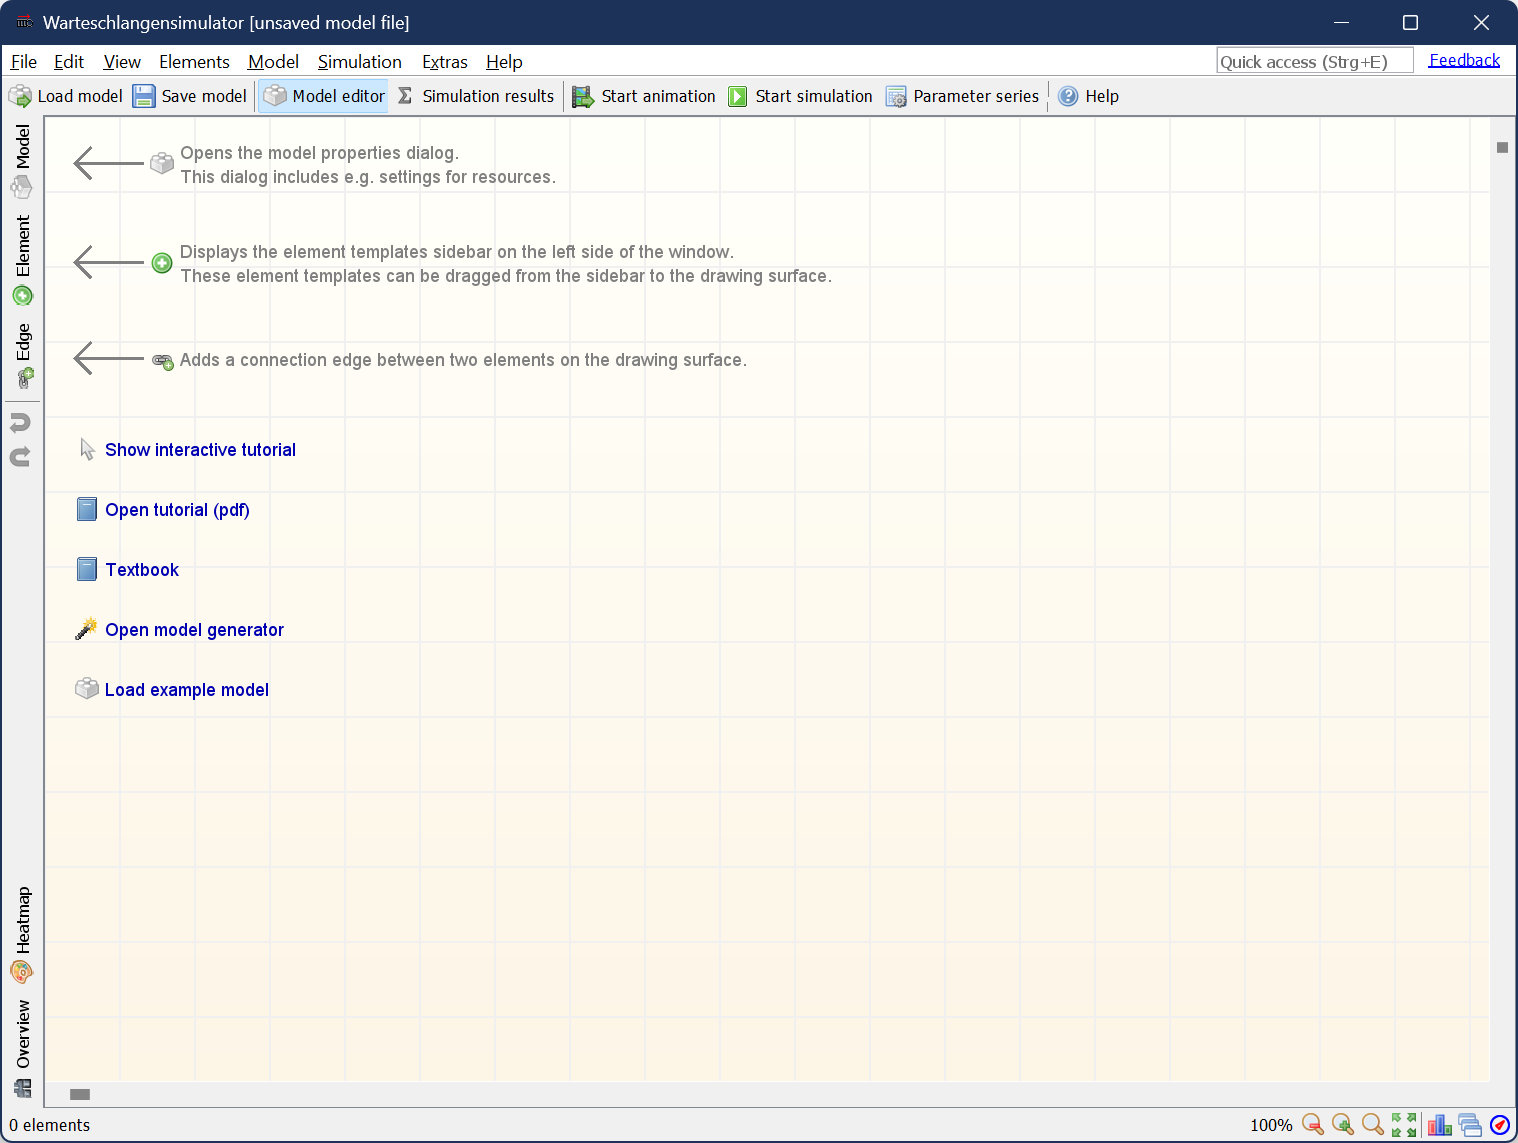
\includegraphics[width=14cm]{ProgramWindow.png}}
	\label{fig:ProgramWindow}
\end{figure}

When starting the program, the drawing area on which the flow chart can be created is displayed directly.

In the upper toolbar, there are the two buttons \textbf{Model editor} and \textbf{Simulation results}, which can be used to switch between the two main program functions:

\begin{itemize}
\item
The \textbf{model editor} contains the drawing surface on which the simulation model can be modeled as a flow chart. In addition, tools for editing the model are displayed via the left toolbar.
\item
The \textbf{simulation results} view is automatically activated after completion of a simulation run and displays the results in the form of texts, tables and graphs. In addition to the possibility to export these individual documents, the simulation results view can also be used to generate reports and to filter the results in a user-defined format.
\end{itemize}



\chapter{The model editor}

The model editor essentially consists of a large drawing surface that occupies almost the entire area of the program window. In addition to this, there is a vertical toolbar on the left-hand side of the window. This toolbar allows to insert elements and connecting edges into the simulation flow chart and to make general settings for the model.

\section{Vertical toolbar}

The three main buttons in the vertical toolbar are:

\begin{itemize}
\item
\textbf{Model:}\\
Clicking this button opens a dialog in which various settings for the simulation model can be made (simulation runtime, available resources, properties of the simulated clients, etc.).
\item
\textbf{Element:}\\
By clicking this button, you can expand and collapse the element templates panel at the left side of the window. You can drag and drop elements onto the drawing surface from this template panel.
\item
\textbf{Edge:}\\
A simulation flow chart consists of two types of objects: elements (also called stations) at which actions take place, and connection edges between the stations. The elements can be dragged from the foldout element template panel to the drawing surface at any point and later moved as desired. There are initially no restrictions: elements can theoretically overlap - which of course would make the model unclear - or be very far apart from each other. Edges, on the other side, cannot exist independently. An edge always connects two elements. Edges are displayed as arrows. This means the direction from an output to a target element is always predetermined. Since edges always have to be connected to elements, they cannot simply be dragged from the templates panel onto the drawing surface, but the start and destination element of an edge always have to be defined. If the edge button is clicked, it remains highlighted until it is clicked again to deactivate the function. As long as the edge function is activated, edges can be inserted into the model by clicking on the source and the destination element one after the other. Whether the element, which is hovered with the mouse, can be used as s source or a destination element, the mouse pointer changes its form to show this.

\end{itemize}

\section{Darwing surface}

Elements which have been dragged from the templates panel to the drawing surface can be moved with the left mouse button pressed.

If several elements are to be moved at the same time, they can be clicked one after the other with the shift key pressed, or a frame can be dragged around them with the left mouse button, in order to select several elements.

Selected elements can be deleted by using the context menu or by pressing the delete key.

Also via the context menu or by double-clicking or by pressing the Ctrl+Return hotkey you can open an edit dialog for all elements, in which the properties of the respective element can be set.

Instead of using the mouse, selected elements can also be moved using the cursor keys: If the Alt key is pressed, the selected elements can be moved with the cursor keys on the drawing surface. When moving elements, they are usually aligned on a grid. If the Shift key is also held down, the elements can be moved pixel by pixel.



\chapter{Presentation of a simple queueing model}

The simplest possible queueing model consists of three elements:

\begin{itemize}
\item
A source,
\item
•	a process station and
\item
an exit.
\end{itemize}

These three elements can be dragged from the template panel on the left side of the window to the drawing surface (if necessary, click on the element button to display the sidebar). Afterwards, the elements can be connected via the edge button: To do this, first click on "Edge" to activate the insertion of connection edges. Then, click on the source element, then click on the process station to insert the first edge, and then on the process station and then on the exit on the drawing surface to insert the second connection edge.
 
\begin{figure}[H]	
	\caption{Simple queueing model in the model editor}
	\centerline{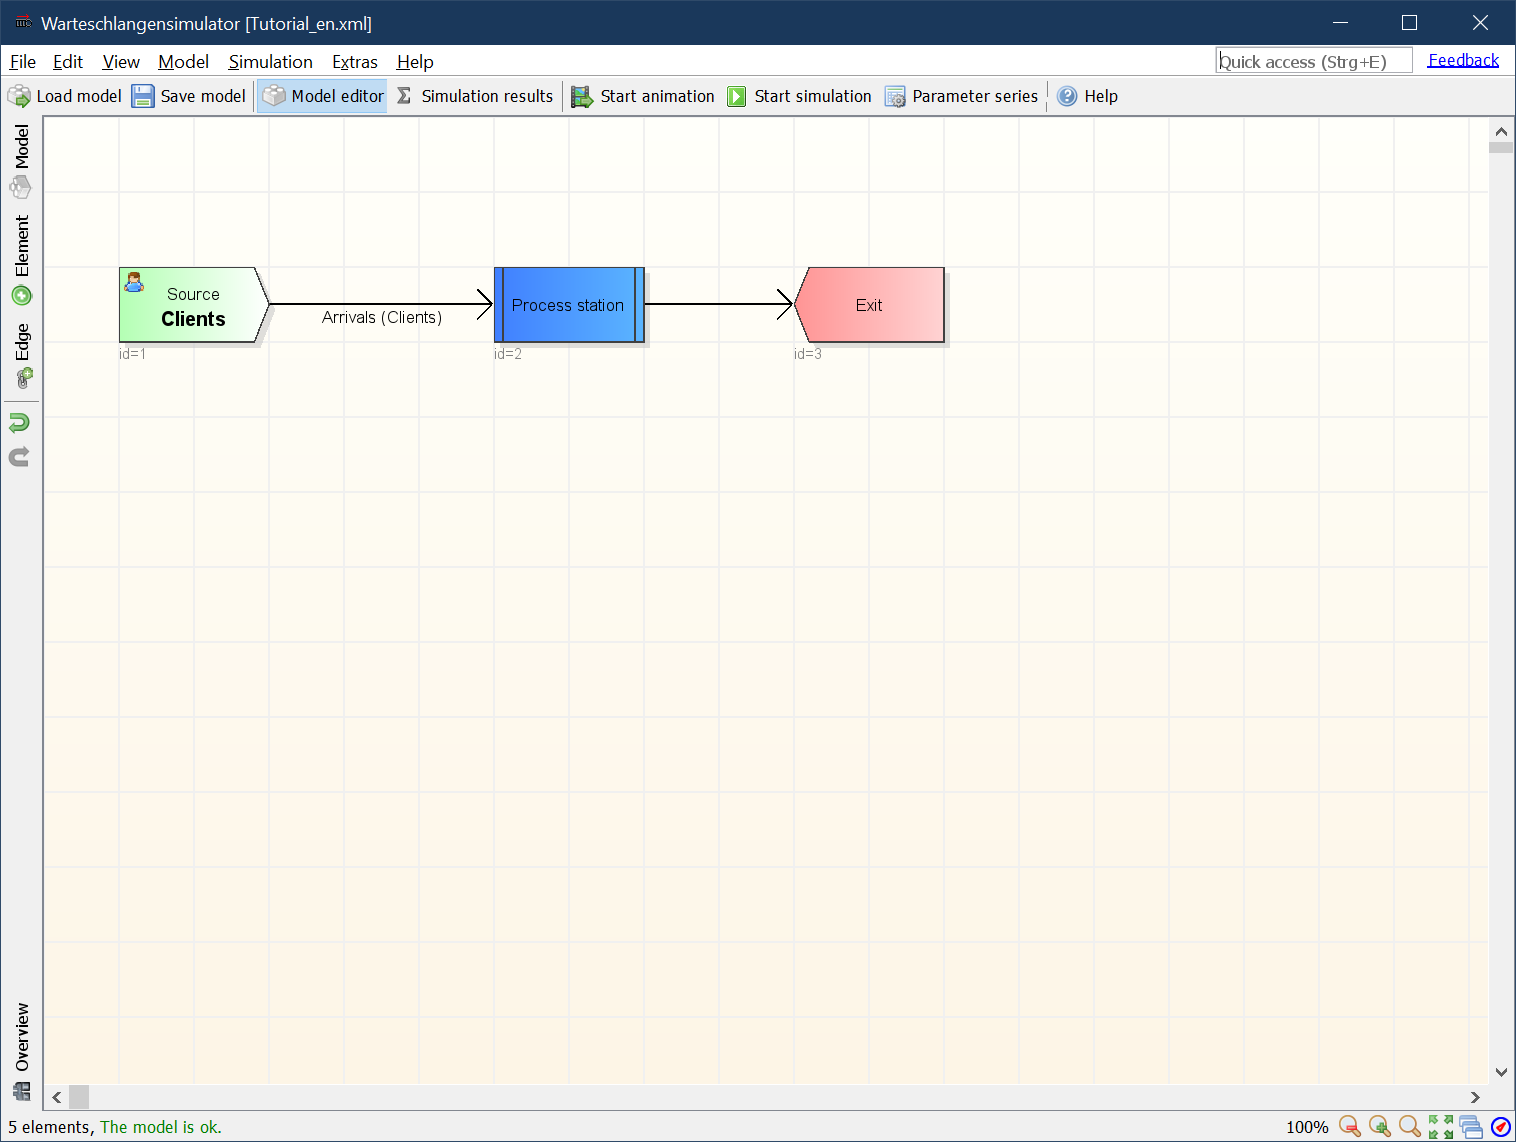
\includegraphics[width=14cm]{ProgramWindowModel.png}}
	\label{fig:ProgramWindowModel}
\end{figure}

The path of the clients through the system always begins at a source and always ends at an exit element. While the exit has no other configuration options, the client source and the process station have to be configured in the following in order to simulate the model.

\section{Configuration of the clients source}

\begin{wrapfigure}{l}{2.25cm}
\vspace{-22pt}
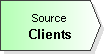
\includegraphics[width=2cm]{IconSource.png}
\vspace{-22pt}
\end{wrapfigure}
Double-clicking on the client source element opens the settings dialog for this element.

\begin{figure}[H]	
	\caption{"Edit source" dialog}
	\centerline{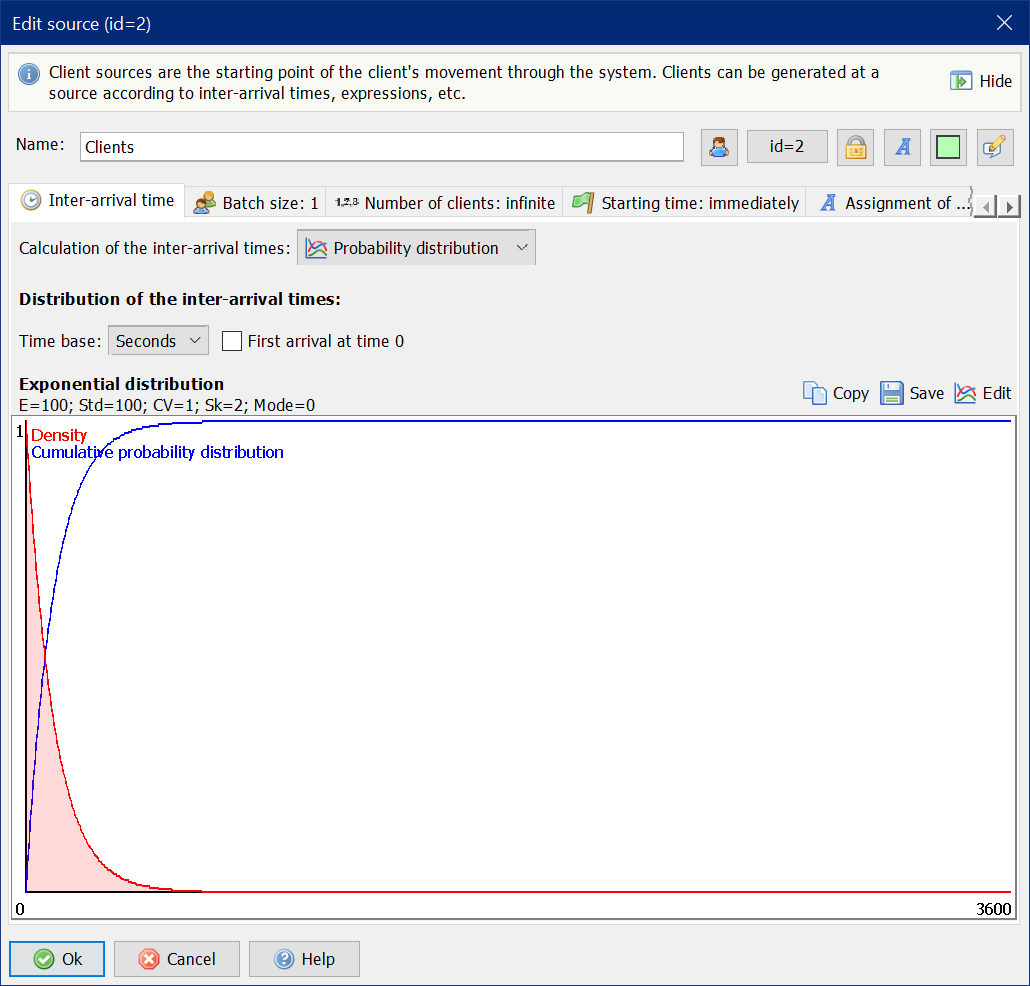
\includegraphics[width=10cm]{DialogSource.png}}
	\label{fig:DialogSource}
\end{figure}
 
In the \textbf{Name} field, the client type of the clients, which are generated in this source, can be set. In the statistics, the performance indicators of the clients generated at this station are identified by this name. The client source generates clients until the end of the simulation (unless otherwise specified) and leads them by the output edge to the next element (in the case of this simple example to the process station).

The arrival times of the clients are determined by means of the inter-arrival times, i.e. the times between the arrivals of two consecutive clients. The inter-arrival times can be determined in the client source element in different ways: via a probability distribution, an expression whose value is recalculated after each client arrival and for which the current system state can be accessed, via a schedule, by a condition which has to be true for a new client arrival, or by one or more signals which trigger client arrivals. For the current example, the default setting to \textbf{determinate the inter-arrival times by a probability distribution} can be kept. Under the field to select the inter-arrival time type the density and the distribution function are displayed if a probability distribution is used. The \textbf{Edit} button opens the distribution editor in which the distribution can be configured. For this model, as inter-arrival time distribution, the exponential distribution should be used with an average distance between two client arrivals, of 60 seconds.

The other dialog elements in the "Edit source" dialog can be used to specify whether clients should arrive individually (default setting) or in groups. It can also be stated that the client source is to generate only a limited number of clients. For this first model, the settings in these areas can be kept without changes.

\section{Configuration of the process station}

\begin{wrapfigure}{l}{2.25cm}
\vspace{-22pt}
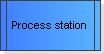
\includegraphics[width=2cm]{IconProcess.png}
\vspace{-22pt}
\end{wrapfigure}
The process station is the central element in most queuing models. For the process station a settings dialog can be opened by double-clicking on the station element, too.

\begin{figure}[H]	
	\caption{"Edit process station" dialog}
	\centerline{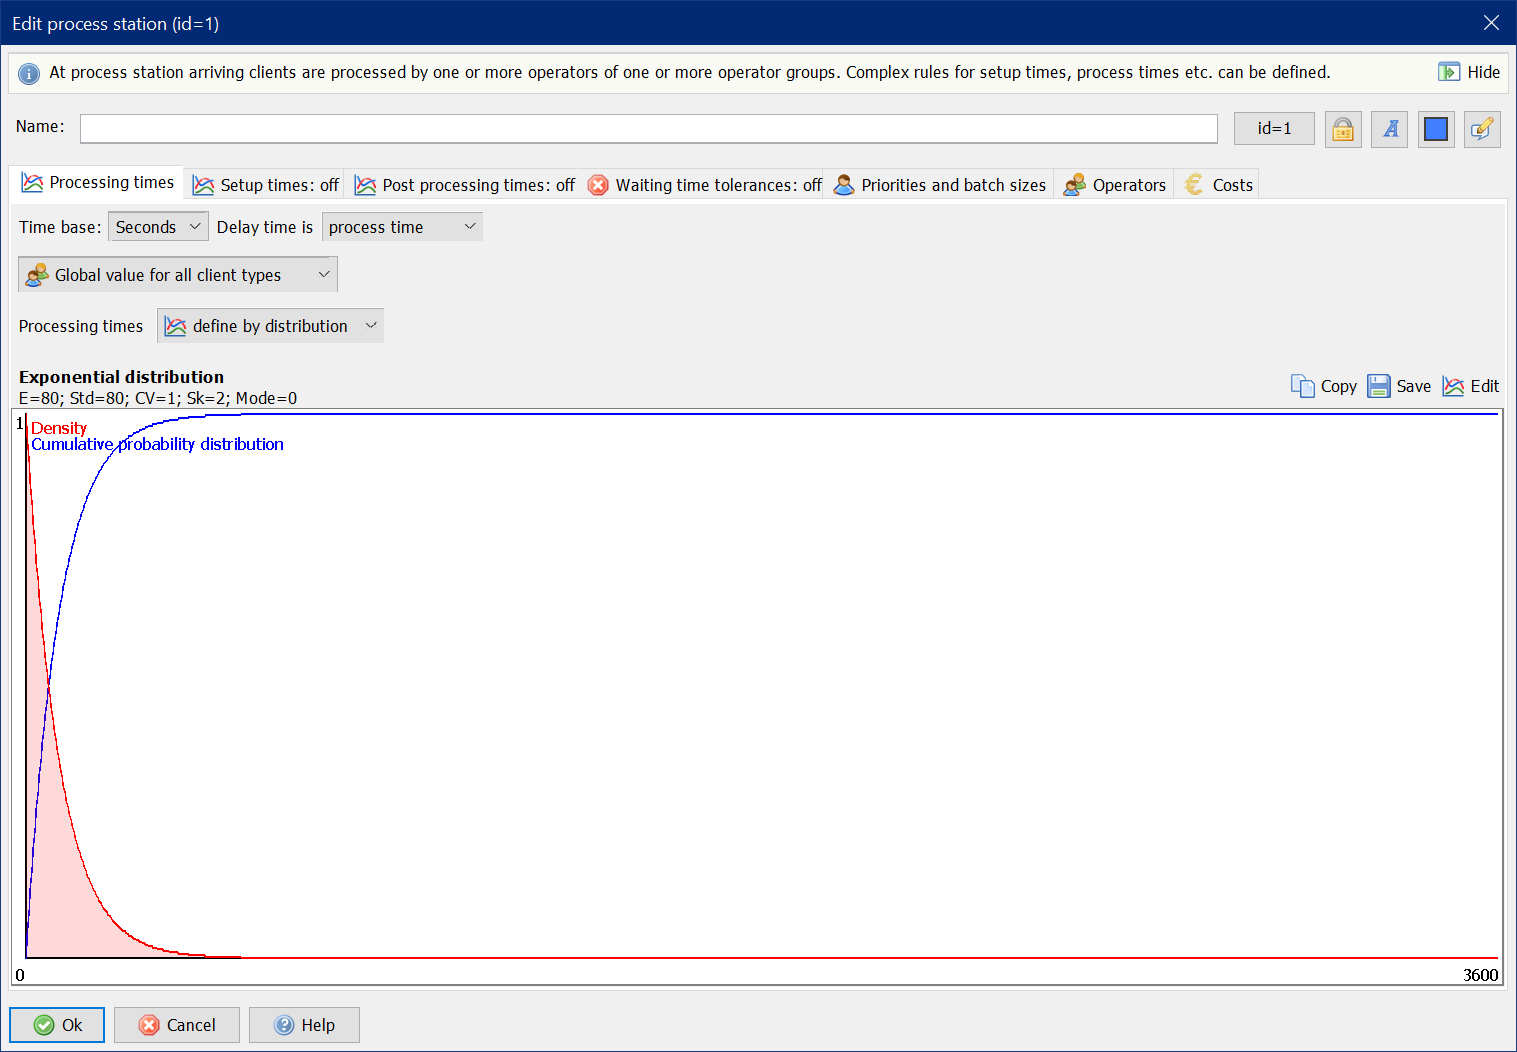
\includegraphics[width=14cm]{DialogProcess.png}}
	\label{fig:DialogProcess}
\end{figure}
 
The name of the process station has no meaning for the simulation. More important are the settings that can be made via the tabs under the name field.

\begin{itemize}
\item
\textbf{Processing times:}\\
On this dialog page the duration of the client’s service process can be defined. The processing times can be defined via a distribution function or via an expression whose value is recalculated during each service process and in which the current system state can be accessed. When using a distribution function, all the usual probability distributions are available. (The function can be edited via the "Edit" button). Since a one-point distribution is also available, deterministic operating times can also be specified. The combo box "\textbf{Processing times}" can be used to set whether the processing times at this station are to be counted as process times, as a transfer times or optionally also as a waiting times in the statistics. This allows mapping the transfer times between stations: By placing pseudo process stations using transfer times between the regular process stations the transfer of the clients can be modeled. On defining the processing times it has to be ensured that the operators are able to handle the incoming clients (by means of average values). In the current example, an average inter-arrival time of 60 seconds was selected. The mean for the processing times is 50 seconds, which means that the operator is fast enough (on average) to serve the incoming clients.
\item
\textbf{Setup times:}\\
On this dialog page, additional times between the service processes of clients of the same or - which is usually the case - of different types can be defined. These setup times, which are optional for each client type transition, can be defined each using either a probability distribution or an expression.
\item
\textbf{Post processing times:}\\
After each service process, a so-called post-processing phase can follow for the operator before he is available again for processing the next client. During the post-processing time, the client is no longer at the process station, that is, the post-processing time has no meaning for him. However, by the post-processing times, the available operating performance is reduced. If an operator requires an average of 60 seconds of operating time and 30 seconds of post-processing time per client, the operator cannot serve 60 clients per hour on the average, but only 40. In this first example, no post-processing times are used.
\item
\textbf{Waiting time tolerances:}\\
The clients can have a limited waiting time tolerance. If the “clients” are workpieces in a production process - and these workpieces are not perishable - an unlimited waiting time tolerance can be assumed. In the case of human clients or the processing of perishable goods, however, one has to assume that they are only ready to wait for a limited time. On the dialog page "Waiting time tolerances" the probability distribution or the expression by which the waiting time tolerance of the clients is determined can be defined. If a process station uses waiting time tolerances, the element needs to have two output edges: one for the successfully served clients and one for the canceling clients. In this first example, no waiting times tolerances are to be modeled.
\item
\textbf{Priorities and batch sizes:}\\
If clients of different types arrive at a process station, it may is desired to prioritize them differently. This means to serve the clients of some groups with a higher priority. On this dialog page, a formula can be specified for each client group, according to which their priority is determined. In these formulas, the variable "w" stands for the client's previous waiting time. If "w" is used as the formula, the first-come-first-serve principle is used: The client who is waiting for longest time is served next. It can also be set up that the customers are not served individually, but in groups (in so-called batches). If a batch size of 2 is set and a single client arrives at an empty process station he has to wait until a second client has arrived. The operating time of the two clients together then corresponds to the processing time indicated on the first dialog page, i.e. the two clients are served simultaneously and not one after each other. In this example, the first-come-first-serve mode, i.e. "w" as a priority for the clients, as well as a batch size of 1, i.e. serving individual clients, should be kept.
\item
\textbf{Operators:}\\
The operators are the most important element of a process station. Various combinations which mostly cannot be mapped by analytical queueing models can be used in the process station. Several operators may be required to perform a service process, and at the same time, several operators may be available. The operators are subdivided into several groups. The necessary and the available number of operators can vary per group. Furthermore, several different process stations can use the same operating groups. Thus, in a canteen model, e.g. the "Food A", "Food B", and "Food C" stations each require the "Operator A", "Operator B" or "Operator C" resource (of which each one is available) but also "Soup ladle", of which a total of only two are available for all stations together. In addition, different alternatives how a client can be served can be defined. This way it is possible to define both and links ("Resources A and B have to be available."), as well as or links ("A client can be served by operator A or operator B."), and both variants can be combined.

The \textbf{resource priority} can be used to set the priority with which certain stations should be given access to the resource when multiple requests are made to a resource at the same time. The higher the priority, the higher the probability that a station will receive the resource. The resources are only reserved if all necessary resources are available at the same time. In this way, deadlock situations are avoided. (It cannot happen that "food dispenser A" has already reserved the "soup ladle" and "food dispenser B" has locked "roasting skewer", but to serve a client at one of the stations both are necessary and both stations mutually block each other.)

To serve a client, at least one operator group has to be defined in the process station. The operator groups can be configured in detail via the model properties dialog. However, new operator groups can also be created directly via the operator station dialog. Click on the "\textbf{Add needed operators group}" button. A dialog appears in which you can set whether an already existing operators group is to be used at this station or whether a new operator group is to be created. As there are no operators groups in the system now, only the option to create a new group is offered. New groups always consist of one operator (which can be changed via the model properties dialog). In the present example, the average intermediate arrival time is 60 seconds, and the average service time duration is 50 seconds, i.e. a group of one operator is sufficient to serve the incoming requests. In the dialog for adding an operator group, a name for the new operator group can optionally be specified (the utilization of the operators is later indicated in the statistics by this name).
\item
\textbf{Costs:}\\
The cost of servicing a client (or a client group in the case of batch processing) can be set as a value per client and / or per service and per post-processing hour on the cost page of the process station edit dialog. These costs are the costs from the point of view of the process station itself. Costs on the client side (cost per waiting, transfer and service second) as well as costs for the operators (costs per availability hour, per hour worked and per idle hour) are defined in the model properties dialog. Costs can also be negative in principle; in this way profits can be mapped. Costs or gains (for example, if a client exits the system successfully served) can be directly represented via the cost element at any point in the flow chart.
\end{itemize}



\chapter{Simulation and statistics output}

By following the steps above this first model should already be operational. If you do not want to create a model but still want to try the next steps, you can also load a model into the editor using the File|Load example|Erlang-C comparison model menu item. This model equals the model described above with the exception of some other intermediate arrival and operating times described above.

By clicking the \textbf{Start simulation} button in the upper toolbar or by pressing the F5 key, the simulation of the model can be started. If you have forgotten to link one station to another, or if you have a misconfiguration that prevents the simulation of the model, an error message will appear and explain the location of the error. The individual stations are identified by their IDs. The IDs of the stations are displayed in the context menu of the respective element, in the title of the respective edit dialog, and as a tooltip when you hover the mouse pointer over the stations. For larger models, you can also use the Find element by ID function from the View menu to find a specific item.

The default number of client arrivals is 10,000,000. (This can be changed via the model properties dialog.) Because the program has will parallelize the simulation by default (if not turned off) across all CPU cores, the simulation process will take about 2 to 10 seconds depending on the performance of the system.

After completing of the simulation, the program automatically switches to the "\textbf{Simulation results}" page. Using the two buttons "Model editor" and "Simulation results" in the upper toolbar, you can switch between the model editor and the simulation result view at any time.

\begin{figure}[H]	
	\caption{Simulation results view}
	\centerline{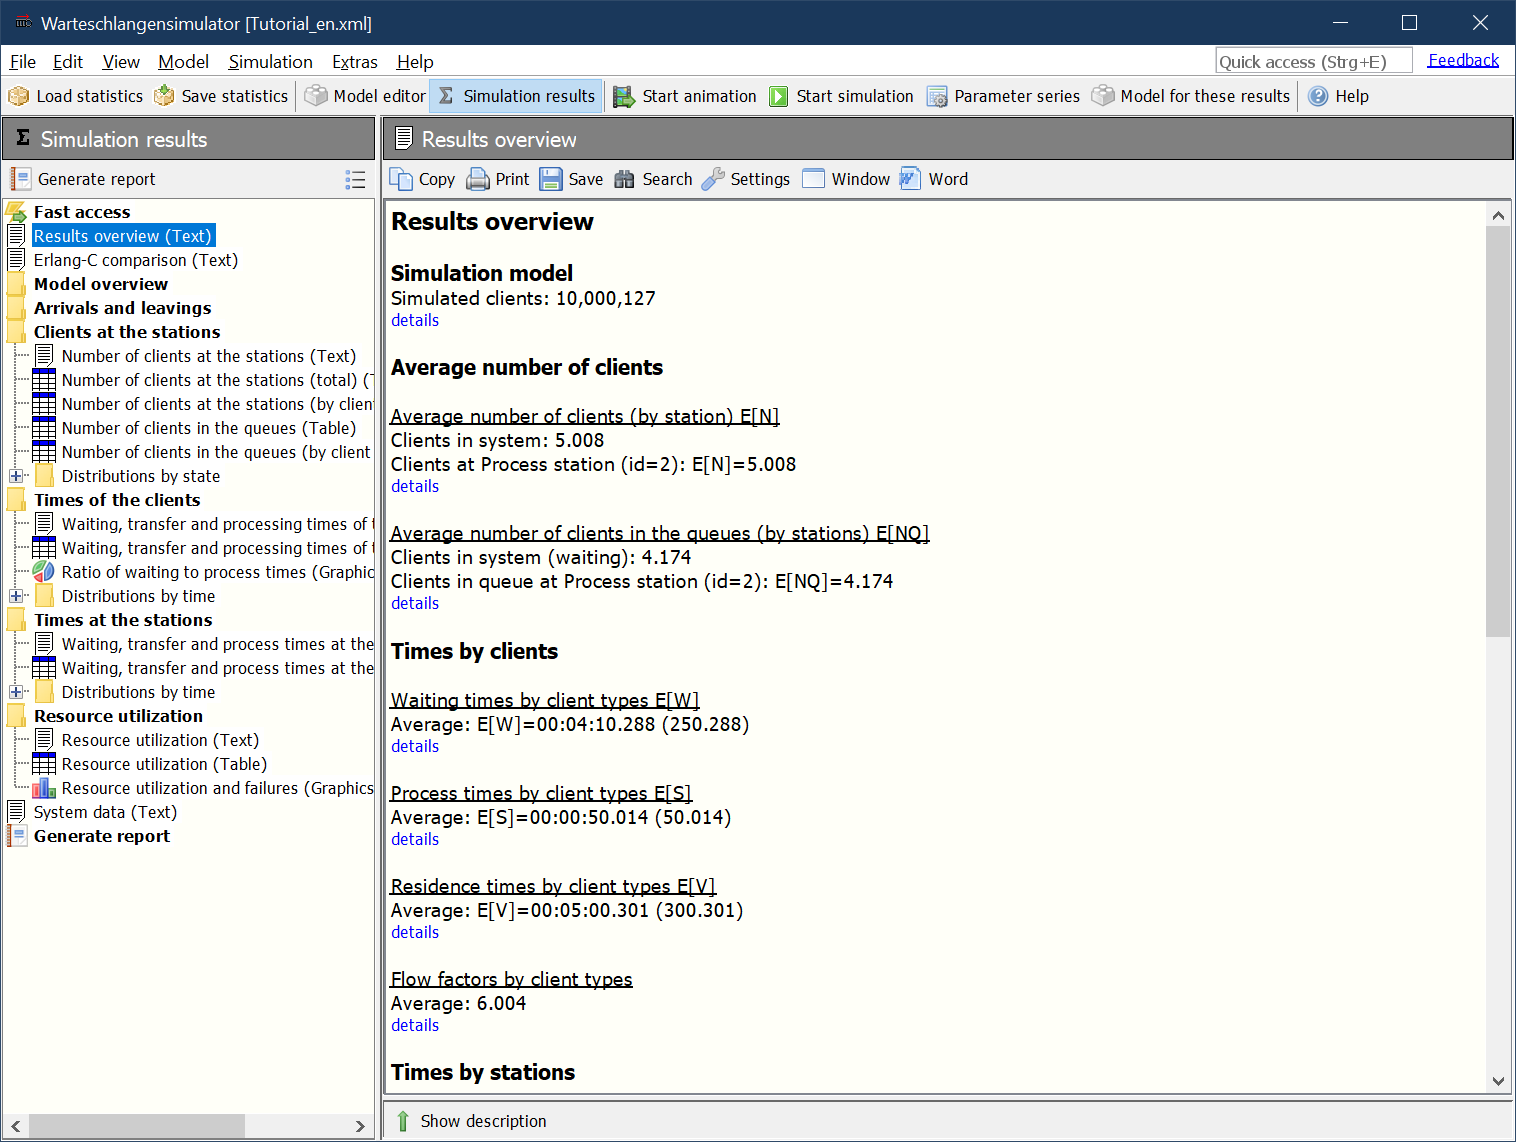
\includegraphics[width=14cm]{ProgramWindowResults.png}}
	\label{fig:ProgramWindowResults}
\end{figure} 

The simulation results page consists on the left side of a tree structure in which the desired data can be selected and on the right side a content area for the respectively selected information. By default, the "Results overview" page is displayed, on which the most frequently required information can be found. The average number of clients in the system and in the queues, as well as the average waiting and service times and the utilization of the operator groups, are displayed here.

The data from each page can be exported by means of the buttons "Copy", "Print" and "Save". Depending on the information displayed (text, table or graphic) various formats including Word documents, Excel tables and pdf files are available for saving.

The first and the last entry in the tree structure on the left side of the window are of particular importance: The \textbf{Fast access} (first entry in the tree structure) allows you to define your own output formats using simple Javascript commands. In this way, if a whole series of models are to be simulated one after the other, always the information which are relevant for the examination can be displayed in the necessary form. You can use the Generate report entry at the bottom of the tree structure to create reports that contain multiple individual documents. As output formats docx, pdf and html files are available. Furthermore, all table information that is retrievable in the tree structure can be stored as worksheets collected in one Excel workbook.

If the simulation results view is active, in the upper toolbar the button \textbf{Model for these results} is available. This button can be used to display the model underlying the simulation results at any time. The idea is as follows: If the results of a simulation are stored, the complete model is stored in the statistics file. In this way, when the statistic results have been loaded back into the simulator, it is always possible to determine the corresponding model to the results, i.e. a separate documentation of models and results is not necessary. The simulation results always contain the models. If you click on the "Model for these results" button, a model editor will open in read-only mode in a new window. Thus, the model can be viewed directly. If the model is to be used as a basis for further simulations, it can be loaded from this model view window via the \textbf{Load model to editor} button at any time in the normal model editor again.



\chapter{Animation}

The animation function, which can be started via the corresponding entry in the horizontal toolbar ("\textbf{Start animation}") or via the F6 key, is used to visualize the processes in the simulation model.

The simulation core of Warteschlangensimulator is primarily designed for the classical simulation for generating statistical data and not directly for the animation. In the event-oriented stochastic simulation, events are processed sequentially; in the simulation process, only the times at which an event occurs exist. Therefore, adjustments have to be made by the simulator in order to simulate a continuous flow during the animation. The animation e.g. is artificially slowed down if there is a longer temporal distance between two events. However, in order to represent a liquid animation, this mapping of the model time to the real time is nonlinear. Due to the sequential processing of the events, it can also occur that the movement of two clients, which actually move at the same time, is displayed one after the other.

\section{Special elements for animation}

In the elements templates panel, the "Animation" section contains some special elements for visualizing certain properties. During a normal simulation, these elements have no meaning. Only in animation mode, these special properties will be visible. The animation elements allow certain parameters (e.g., current utilization, client waiting times, etc.) to be represented as numbers, bars, diagrams, or even in the form of a traffic light.

The values to be displayed are defined in the form of formulas. The station data is accessed by the IDS of the stations. For example, "WIP(2)" gets the current number of clients (work units in process) at the station with ID 2.

Clients are identified by the ID of the station where they were generated. For example, "WaitingTime\_avg(1)" gets the average waiting time of the clients of the type generated at the source with ID 1. The calculation is based on clients type and the name of the station is only exemplary. If there are two sources that generate clients of the same type, the average waiting time is output by the clients of the two client sources.
 
\begin{figure}[H]	
	\caption{"Edit expression" dialog}
	\centerline{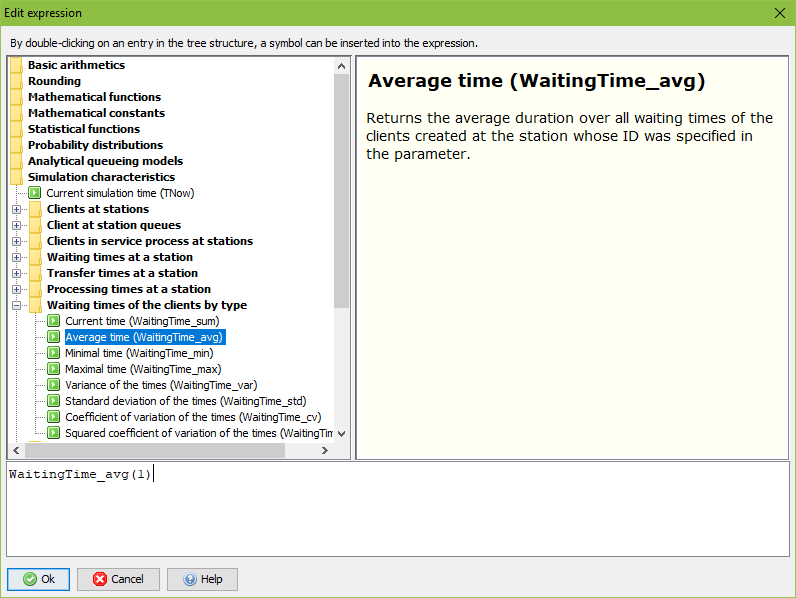
\includegraphics[width=14cm]{DialogExpressionBuilder.png}}
	\label{fig:DialogExpressionBuilder}
\end{figure} 

A list of all available commands can be displayed in the "Edit Expression" dialog, which can be called via the \textbf{magic wand icon} on the right of all formula input fields.

\section{Recording animations}

You can record animations as avi video files via the \textbf{Simulation|Record animation} menu item. Because Warteschlangensimulator uses the mjpeg codec to store images (unlike real-video video codecs with use key frames and intermediate images), the video files are relatively large.



\chapter{Model properties}

If the model editor is active, the model properties dialog can be accessed via the "Model" button in the vertical toolbar on the left side of the program window.
 
\begin{figure}[H]	
	\caption{"Model properties" dialog}
	\centerline{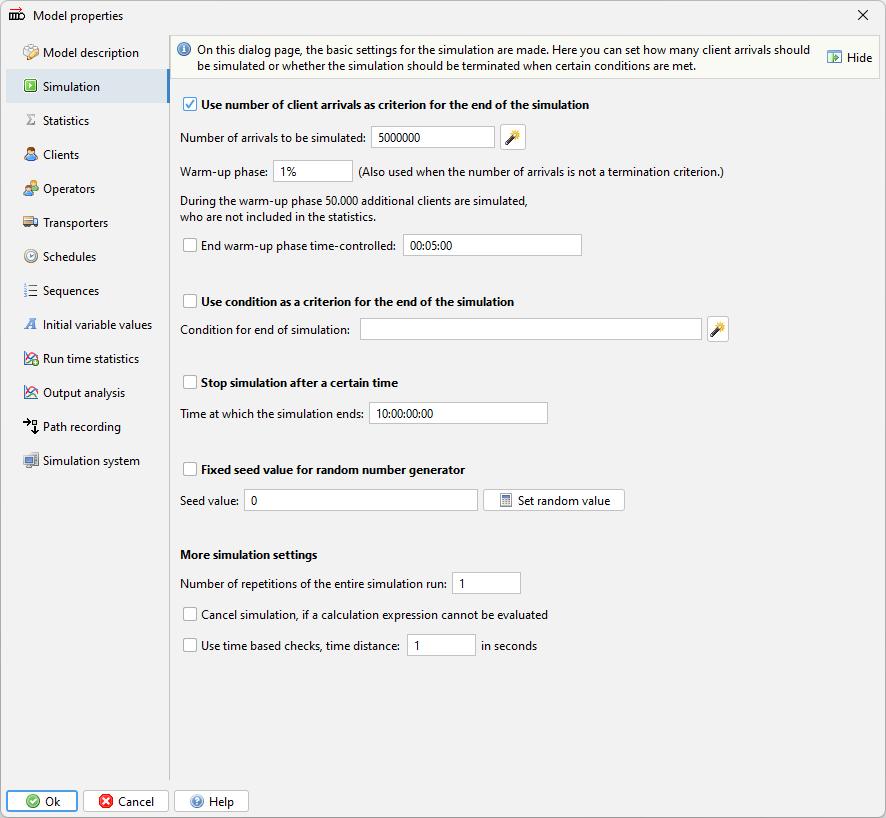
\includegraphics[width=14cm]{DialogModel.png}}
	\label{fig:DialogModel}
\end{figure} 

This dialog contains several tabs:

\begin{itemize}
\item
\textbf{Model description:}\\
On this page a description of the model can be entered. This description has no meaning for the simulation, but it is stored together with the simulation model and can be used for identifying the model or later to understand the meaning of the model.
\item
\textbf{Simulation:}\\
This dialog page can be used to define the simulation run time. By default, the simulation is executed one time and is terminated when a certain number of clients have passed through the system (the default value is 10,000,000). Alternatively, a termination condition which is continuously checked during the simulation or a termination time (measured in the time in the simulation) can be specified.

Furthermore, this page can be used to determine how long the warm-up phase (which is also called the transient phase) should take. A warm-up phase of 1\% with a total of 5,000,000 simulated clients means that a total of 5,050,000 (= 5,000,000 $\cdot$ 101\%) clients are simulated. However, the recording of the statistic results starts only from the 50,001th client. This way, the statistic effect of edge effects can be eliminated.

Optionally a fixed seed value for the random numbers generation can be defined. This is particularly interesting for the animation of models. If using a fixed seed value is active, exactly the same sequence of pseudo-random numbers is used with each start of simulation or animation. In this way, exactly reproducible results can be achieved. However, since the use of a fixed seed value for the random number generation prevents the simulator from parallelizing the simulation over several CPU cores, it should only be activated if the effect of exactly the same pseudo-random numbers is really needed.
\item
\textbf{Clients:}\\
On the Clients dialog page of the model properties dialog, all client types that are defined in the model are listed automatically. For each client type properties which are relevant for the animation (type of icon representing the clients of the type) and for the statistics (color of the bars for the respective client type in the statistics) can be set up. Additionally the costs per waiting, transfer and service second for the client can be defined.
\item
\textbf{Operators:}\\
On this page the operator groups in the model can be defined. Practically, the "operators" can be any resources necessary for the process that can be any certain tools that are required in the manufacturing process, etc. When configuring a process station, an operator group is often created directly. In the settings dialog of the process station, however, only the name of the new operator group can be defined. In the model properties dialog, you can specify the number of operators in the respective groups (in addition to a fixed number, the option "infinite number" or the specification of a schedule is also possible) and the cost per availability hour, per hour worked and per hour Idle hour. The distinction between availability hour and worked hour is particularly useful for machines, which use electricity: By defining a cost value for the availability hours may rental costs for the machine can be displayed. The costs for the worked time reflect the electricity costs to be accrued thereon. In addition, the system can be used to define failures or breaks: An operator can enter a break after a certain number of service processes, after a certain presence time or after a certain actively worked time.
\item
\textbf{Transporters:}\\
Transporters are used to carry client from Transporter start to Transport destination stations. Transporters behave similar to resources. But in contrast to resources they have a defined location. This means the transporting times need not to be defined by distributions by are calculated from the distance between origin and destination station. (A distance matrix for all origin and destination stations can be set up per transporter type.) Additionally
loading and unloading times which apply if the transporter was carrying clients can be defined per transporter type.
\item
\textbf{Schedules:}\\
Schedules can be used to describe inter-arrival times between clients  at the source stations as well as the availability of operators. The time slot lengths one minute, 15 minutes, 30 minutes, one hour and one day are available as basis for the time slots within the schedule. For each time slot, an individual value can be set which indicates how many clients should arrive in this time segment or how many operators of the respective type shall be available in the time slot. Schedules can be of any length. In addition, you can set how to proceed at the end of the defined schedule: The schedule can be continued with zeros, can remain at the last value, can be repeated from the beginning, or can be continued with zeros until the end of the current day then be restarted.
\item
\textbf{Sequences:}\\
Sequences can be used to define production plans which can be used in combination with transport elements. Clients can be transported between transport origin and transport destination stations in two ways: Either the information clients of which type are to be transported to which destination station is stored directly at the origin station or the information which client is to be routed to which destination is stored at the client object by means of a client assigned production plan.
\item
\textbf{Initial variable values:}\\
Variables which are used in the simulation process can be assigned initial values on this dialog page. These initial values apply immediately from the beginning of the simulation on. In this way, e.g. constants that are used in different places in calculation expressions can be defined.
\item
\textbf{Run time statistics:}\\
This function allows to define expressions whose value changes over the simulation time and whose current value should be recorded for the statistics.
\item
\textbf{Output analysis:}\\
The simulator offers two functions for the analysis of the simulation results: On the one hand, the autocorrelation of the waiting times can be determined during the simulation (i.e., how often, for example, a long waiting time results in the next waiting times being long, too). This feature normally is turned off because it slows down the simulation. On the other hand, it is possible to set whether, based on batch sizes determined beforehand (by means of autocorrelation analysis), confidence intervals for different parameters should be calculated.
\item
\textbf{Path recording:}\\
As an option, the movement of the clients through the system can be recorded by counting the paths taken or by counting the number of station transistions.
This count slows down the simulation and is therefore deactivated by default. If the counting is activated, the recorded information will be displayed using additional
statistics pages and Sankey diagrams showing the client flows through the system are offered.
\item
\textbf{Simulation system:}
No settings can be made on this dialog page. On this page information about the model are displayed. It is stated if the model contains errors and if the simulation of the current model can be parallelized over all CPU cores. If no, the properties, which prevents this, are listed.

\end{itemize}

\chapter{More elements}

In addition to the previously presented elements for generating (source) and serving (process station) clients and for the clients to leave the system (exit), there are a number of other elements in the template panel that can be used to extend models. The available elements are listed here thematically grouped:

\begin{itemize}
\item
\textbf{Input/Output:}\\
Contains elements that will allow new clients to enter the system and to leave the system at the end of the process.
\item
\textbf{Processing:}\\
Contains the classic elements to serve clients or to delay clients on their way through the system.
\item
\textbf{Assignments:}\\
Allows to assign properties to clients (e.g., a new client type), to change variables or counters or to capture additional costs.
\item
\textbf{Branching:}\\
By using the elements in this section, it is possible to direct clients based on their properties in different directions, or to duplicate clients.
\item
\textbf{Barriers:}\\
Barriers allows to delay clients until certain conditions are met. There are elements that delays clients based on conditions to be tested (in this way, everything can be mapped, but appropriate expressions have to be defined) as well as elements that check the availability of resources as well as classic barriers reacting on signals triggered by signal elements.
\item
\textbf{Batching:}\\
In many production processes, partial production processes are combined into one process, e.g. the station where the engines are installed in the car bodies. The elements in this section allow the mapping of such processes. There are elements in which two client flows are incoming (e.g., "engine" and "empty body"), the clients end their life cycles at that station and instead a new client ("body with engine") is created and forwarded. At another station, a fixed number of (potentially similar) objects arriving over a common line can be grouped into a batch or a new object. The connection of the elements may be temporary (i.e., later resolvable) or permanent.
But for simple batch operation at a process station, the clients do not need to be batched in advance at all. The batch operation of individually incoming clients can be defined directly in the process station element.
\item
\textbf{Transport:}\\
Via the transport elements, clients can be transported from one station to another station, which is not connected to the source station. For the necessary transport time, a time period can be set up individual per transport destinations, which are determined according to the respective client type or also by an expression.
\item
\textbf{Data input/output}:\\
By using the input elements numerical values can be read from files or database tables and used for variable assignment.
Log file entries can be generated and stored to files and database tables at any time via the output elements in the simulation process.
\item
\textbf{Flow control logic:}\\
The flow control logic elements allow to implement some flow control (consisting of conditional branching and loops)
like in classical programming languages.
\item
\textbf{Analog values:}\\
By using the elements in this section some continuous changing values can be used in the in general discreet simulation.
\item
\textbf{Animation:}\\
The elements gathered in this section allow to visualize certain parameters during the animation. The representation of the values can take place in the form of texts, bars, line diagrams or also in the form of a traffic light. These elements have no further meaning for classical simulation.
\item
\textbf{Optical decoration:}\\
The elements in this section have no meaning for the simulation or the animation. The elements are used exclusively for the optical design of simulation models (for example, to display information texts or to highlight certain sections by framing colored boxes).
\item
\textbf{Others:}\\
There is one very special elements in this section: The sub model element allows to package complete sub models into a single station so as to keep the main model clearer.
\end{itemize}

\section{Description of some of these elements}

The complete description of all these elements would be beyond the scope of this introduction, therefore only a few examples are presented in the following section:

\subsection*{Delay element}

\begin{wrapfigure}{l}{2.25cm}
\vspace{-22pt}
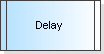
\includegraphics[width=2cm]{IconDelay.png}
\vspace{-22pt}
\end{wrapfigure}
The delay element represents a simpler variant of a process station: There is no queue here. All incoming clients are immediately served. However, no operators are required for this. The clients are simply delayed for a certain time, which can be defined via a probability distribution or an expression. Just as a process station, it can be set, whether the delay time should be recorded as process time, as transfer time or as waiting time in the statistics.

\subsection*{Type assignment element}

\begin{wrapfigure}{l}{2.25cm}
\vspace{-22pt}
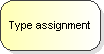
\includegraphics[width=2cm]{IconAssign.png}
\vspace{-22pt}
\end{wrapfigure}
Via the type assignment element, the type of a client (by which his / her data is later recorded in the statistics) can be changed. Each client is already given a certain type by the source. If different control alternatives are to be compared, it can be useful for comparability reasons to supply them with exactly the same client input stream. This is done by doubling the client's incoming stream after production via a duplicate element. In the following, an individual client type can be assigned to each of the two sub-streams via a type assignment element.

\subsection*{Decide element}

\begin{wrapfigure}{l}{2.25cm}
\vspace{-22pt}
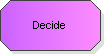
\includegraphics[width=2cm]{IconDecide.png}
\vspace{-22pt}
\end{wrapfigure}
Contrary to most elements, which can take any number of incoming edges, but have only one outgoing edge, any number of edges can lead out of the decide element. The settings dialog of the decide element allows you to specify the criteria according to which the clients are to be directed in the different directions. The following options are available:
\begin{itemize}
\item
Clients can be routed \textbf{randomly} to the different outgoing edges (with a rate for each direction).
\item
Customers may be routed in different directions (e.g., in the direction of the station where the least clients are currently located) according to certain \textbf{conditions} to be tested.
\item
The clients can be branched to the various directions according to the \textbf{type of the clients}.
\item
The clients can be routed to the different edges \textbf{one after each other}.
\item
The clients can be routed to the edges by properties (e.g.\ \textbf{shortest queue length}) of the next stations.
\end{itemize}

\subsection*{Duplicate element}

\begin{wrapfigure}{l}{2.25cm}
\vspace{-22pt}
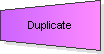
\includegraphics[width=2cm]{IconDuplicate.png}
\vspace{-22pt}
\end{wrapfigure}
The duplicate element also has multiple outgouing edges. In contrast to the decide element, an arriving client is not forwarded via one of the outgoing edges, but copies of the client are created, and an identical client object is forwarded simultaneously over each of the outgoing edges.

\subsection*{Condition element}

\begin{wrapfigure}{l}{2.25cm}
\vspace{-22pt}
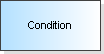
\includegraphics[width=2cm]{IconCondition.png}
\vspace{-22pt}
\end{wrapfigure}
Clients can be delayed by terms of conditions. Clients are only forwarded as long as the specified condition is fulfilled. For example, clients can be delayed until the number of clients in some model section is below a specified threshold value.

\subsection*{Sub model element}

\begin{wrapfigure}{l}{2.25cm}
\vspace{-22pt}
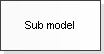
\includegraphics[width=2cm]{IconSubModel.png}
\vspace{-22pt}
\end{wrapfigure}
A complete sub-flow chart can be implemented in a sub model. In this way, larger models can be kept clearer. To the outside, a sub model element looks like a normal element. The properties dialog allows you to set how many incoming and outgoing edges it should accept. If the menu item Edit sub model is clicked in the context menu, or if the key combination Shift + Return is pressed with the sub model element selected, another model editor opens in a dialog. The defined incoming and outgoing edges are shown here as non-erasable pseudo-elements. The sub model can be created between these.

\end{document}